\documentclass [12pt,norsk]{article}

\usepackage [latin1] {inputenc}
\usepackage[norsk]{babel} 
\usepackage [T1] {fontenc}
\usepackage[pdftex]{graphicx}
\usepackage{epstopdf}
\usepackage[vmargin=27mm,hmargin=22mm]{geometry}
\usepackage[usenames]{color}
\usepackage{array,booktabs}
\newcommand{\espen}{Espen L\o kseth} 
\usepackage{amsmath}
\usepackage{hyperref}
\hypersetup{
    colorlinks,
    citecolor=black,
    filecolor=black,
    linkcolor=black,
    urlcolor=black,
	pdfstartview=FitH,
    bookmarksopen=true,
    bookmarksnumbered=true,
	bookmarksopenlevel=2,
    pdftitle =  {Dokument laget av \espen},
    pdfauthor = {\espen},
    pdfproducer={\espen}
    }
\usepackage{datetime}
\usepackage{fancyhdr}


\usepackage{enumerate}
\usepackage{enumitem}
\usepackage{float}
\usepackage{multirow}
\usepackage{clock}

\usepackage{titleref}
\usepackage{sectsty}
\usepackage{lipsum}

\usepackage{chngcntr}


% VIKTIG VIKTIG VIKTIG
\usepackage{subfiles}


% Få nummerering til å inkludere section-nummer
% <section-figurnummer>
\counterwithin{figure}{section}
\counterwithin{equation}{section}
\counterwithin{table}{section}

\renewcommand{\theequation}{\thesection-\arabic{equation}}
\renewcommand{\thefigure}{\thesection-\arabic{figure}}
\renewcommand{\thetable}{\thesection-\arabic{table}}

% For å få luft mellom caption og tabell når caption står over tabellen.
\setlength{\belowcaptionskip}{\abovecaptionskip}



% Stroe bokstaver og Helvetica-font i section
\newcommand{\changefont}[3]{
\fontfamily{#1} \fontseries{#2} \fontshape{#3}
\selectfont}

\sectionfont{\changefont{phv}{bx}{n}\uppercase}
\subsectionfont{\changefont{phv}{bx}{n}}
\subsubsectionfont{\changefont{phv}{bx}{n}}

% Ny side for alle section
\let\stdsection\section
\renewcommand\section{\newpage\stdsection}


% MARGINER :S
\setlength{\headheight}{29mm}
\setlength{\voffset}{-2mm}
\setlength{\headsep}{7mm}
\setlength{\textheight}{200mm}
\setlength{\hoffset}{5mm}
\setlength{\textwidth}{169mm}

% Standardstil
\pagestyle{fancy}






%
%
%\renewcommand*{\refname}{\vspace*{-12mm}}
%\renewcommand*{\bibname}{\vspace*{-12mm}}
%\renewcommand\section{\stdsection}
%%%%%%%%%%%%%%%%%%%%%%%%%%%%%%%%%%%%%%%%%%%%%%%%%%%%%%%%%%%%%%%%%%%%%%%%%%
% Referanser
%%%%%%%%%%%%%%%%%%%%%%%%%%%%%%%%%%%%%%%%%%%%%%%%%%%%%%%%%%%%%%%%%%%%%%%%%%
%\thispagestyle{fancy}{
%\rhead{\ref*{sec:Ref} \nameref*{sec:Ref}}}


%\renewcommand*{\refname}{\vspace*{-12mm}}





%\usepackage{pifont}
%\usepackage{amssymb}
%\usepackage{wrapfig}
%\usepackage{textcomp}
%\usepackage{tikz}
%\usepackage{bbold}
%\usepackage{etoolbox}
%
%\usepackage{esint}
%\usepackage{savesym}
%\savesymbol{iint}
%\savesymbol{iiint}
%\savesymbol{iiiint}
%\restoresymbol{asmath}{iint}
%\restoresymbol{asmath}{iiint}
%\restoresymbol{asmath}{iiiint}



%%%%\usepackage [dvips] {epsfig}
%%%%%\usepackage{graphicx}





%
%\usepackage{savesym}
%\savesymbol{todo} % occurs in both packages
%\usepackage[show]{ed}
%\restoresymbol{ed}{todo} % now available as \edtodo
%\usepackage{todonotes}

%pdfstartview
%Possible values are Fit, to
%show the whole page; FitH, to t the width of the
%page in the window; or FitB, to t the width of the
%contents to the window.
%
%� FitH : Fit whole width of page
%� FitV : Fit whole height of page
%� FitB : Fit whole �Bounding Box� page
%� FitBH: Fit whole width of �Bounding Box� of page
%� FitBV: Fit whole height of �Bounding Box� of page

% Fra Matte III

\newcommand{\Espen}{Espen L\o kseth} 
\newcommand{\FTint}{\ensuremath{\int_{C}{\vec{F}\cdot\vec{T}ds}}}
\newcommand{\Greens}{\ensuremath{\varointctrclockwise_{C}{Pdx+Qdy}=\iint_{R}{\left(\frac{\partial Q}{\partial x}-\frac{\partial P}{\partial y}\right)dA}}}
\newcommand{\parDiff}[2]{\ensuremath{\frac{\partial #1}{\partial #2 }}}
\newcommand{\dparDiff}[2]{\ensuremath{\dfrac{\partial #1}{\partial #2 }}}
\newcommand{\abs}[1]{\ensuremath{\left| #1 \right|}}

\newcommand{\mat}[2][rrrrrrrrrrrrrrrrrrrrrrrrrrrrrrrrrrrrrrrrrrrrrrrrrrr]{\left[\begin{array}{#1}#2 \\ \end{array} \right]}
\newcommand{\detM}[2][rrrrrrrrrrrrrrrrrrrrrrrrrrrrrrrrrrrrrrrrrrrrrrrrrrr]{\left|
\begin{array}{#1}#2 \\ 
\end{array} \right|}
\newcommand{\tekst}[1]{\mathrm{#1}}
\newcommand{\hatt}{\ensuremath{\wedge}}
\newcommand{\linjeR}{\ensuremath{\int_{C}{\vec{F}\,d\vec{r}}}}
\newcommand{\dr}{d\vec{r}}
\definecolor{mblue}{rgb}{0,0.08,0.45}
\definecolor{mgreen}{rgb}{0,0.6,0}
\newcommand{\green}[1]{\textcolor{green}{#1}}
\newcommand{\red}[1]{\textcolor{red}{#1}}
\newcommand{\blue}[1]{\textcolor{blue}{#1}}
\newcommand{\maple}[1]{

		\noindent\newline\textit{Maple:}\\
		\texttt{#1} \newline
}
\makeatletter
\newcommand{\romertall}[1]{\romannumeral #1}
\newcommand{\Romertall}[1]{\expandafter\@slowromancap\romannumeral #1@}
\makeatother
\newcommand{\blankLinje}{\\ \newline}
\newcommand{\blanklinje}{\\ \newline}
\newcommand{\storboks}[1]{\fbox{\parbox{\textwidth}{#1}}\vspace{3mm}}











% Fra Statistikk

\newcommand{\snitt}{\ensuremath{\cap}}
\newcommand{\union}{\ensuremath{\cup}}
\newcommand{\p}[1]{\ensuremath{P\!\left( #1 \right)}}
\newcommand{\ptekst}[1]{\ensuremath{P\!\left(\text{\dq #1\dq}\right)}}

\newcommand{\classpad}[1]{

		\noindent\newline\textit{ClassPad:}\\
		\texttt{#1} %\newline
}
\newcommand{\dsum}{\ensuremath{\displaystyle\sum}}
\newcommand{\dint}{\ensuremath{\displaystyle\int}}
\newcolumntype{x}[1]{>{\raggedright}p{#1}}
%\newcolumntype{x}[1]{>{\raggedleft}p{#1}}

\newcommand{\losning}{\noindent\newline
        \textit{L�sning:}\\}
        
\newtimeformat{tidsformatTall}{\twodigit{\THEHOUR}.\twodigit{\THEMINUTE}}
\newdateformat{datoformatTall}{\twodigit{\THEDAY}.\twodigit{\THEMONTH}.\THEYEAR}

\newcommand{\talldato}{\datoformatTall\today}
\newcommand{\tallklokke}{\tidsformatTall}

\newcommand{\sistKompilert}{\footnotesize\sffamily
    Sist kompilert \talldato{ } kl. \tallklokke \normalfont\normalsize}

%\newcommand{\N}{\ensuremath{\text{N}}}
\newcommand{\N}[1]{\ensuremath{\text{N}\!\left(#1\right)}}
\newcommand{\Bin}[1]{\ensuremath{\text{Bin}\!\left(#1\right)}}
\newcommand{\Hyp}[1]{\ensuremath{\text{Hyp}\!\left(#1\right)}}
\newcommand{\Poisson}[1]{\ensuremath{\text{Poissin}\!\left(#1\right)}}
\newcommand{\Geo}[1]{\ensuremath{\text{Geo}\!\left(#1\right)}}





% Fra kybernetikk

\newcommand{\Mat}[2][ccccccccccccccccccccccccccccccccccccccccccccc]{\left[\begin{array}{#1}#2 \\ \end{array}\right]}
\newcommand{\sq}{\textquotesingle} %For Maple og MATLAB!!!
\newcommand{\bs}{\textbackslash{}} 


%Diverse
\newcommand{\pref}[1]{\hyperref[#1]{(\ref*{#1})}}
\newcommand{\vfantom}[1]{\vphantom{\rule{0pt}{#1}}} 


% Fra matte 4
\newcommand{\Lap}[1]{\ensuremath{\mathcal{L}\left\{#1\right\}}}
\newcommand{\Fou}[1]{\ensuremath{\mathcal{F}\left\{#1\right\}}}




% Fra Industielle programmeringssystemer
\newcommand{\reff}[1]{\hyperref[#1]{figur\,\ref*{#1}}}
\newcommand{\refb}[1]{\hyperref[#1]{figur\,\ref*{#1}}}
\newcommand{\reffo}[1]{\hyperref[#1]{formel\,(\ref*{#1})}}
\newcommand{\reft}[1]{\hyperref[#1]{tabell\,\ref*{#1}}}
\newcommand{\refv}[1]{\hyperref[#1]{vedlegg \ref*{#1}}}

\newcommand{\refF}[1]{\hyperref[#1]{Figur\,\ref*{#1}}}
\newcommand{\refB}[1]{\hyperref[#1]{Figur\,\ref*{#1}}}
\newcommand{\refFo}[1]{\hyperref[#1]{Formel\,(\ref*{#1})}}
\newcommand{\refT}[1]{\hyperref[#1]{Tabell\,\ref*{#1}}}
\newcommand{\refV}[1]{\hyperref[#1]{Vedlegg \ref*{#1}}}




\newcommand{\Referanser}[1]{\clearpage
\let\a\refname
\renewcommand*\refname{\MakeUppercase{\a}}
\thispagestyle{fancy}{
\rhead{\a}}
\phantomsection
\addcontentsline{toc}{section}{\a}
}

\newcommand{\Vedlegg}[1]{\clearpage
\thispagestyle{fancy}{
\rhead{\currenttitle}}
\phantomsection
\addcontentsline{toc}{section}{Vedlegg}
\section*{Vedlegg}}




\newcommand{\RapportFra}{\textbf{\MakeUppercase{Rapport fra 6.-semestersprosjekt våren 2011}}}
\newcommand{\Gruppe}{IA6-11-11}
\newcommand{\Emne}{Industrielle programmeringssystemer}
\newcommand{\Emnekode}{IA3106}
\newcommand{\Tittel}{Fyllestasjon for bokser vha. vision-kamera}
\hypersetup{pdftitle ={\Tittel},
            pdfauthor={\Gruppe{} ved \HiT}}

\newcommand{\Hovedveileder}{Morten Pedersen}
\newcommand{\Biveileder}{}
\newcommand{\Sensor}{}
\newcommand{\Prosjektpartner}{}




\begin{document}
%%%%%%%%%%%%%%%%%%%%%%%%%%%%%%%%%%%%%%%%%%%%%%%%%%%%%%%%%%%%%%%%%%%%%%%%
% Forside
%%%%%%%%%%%%%%%%%%%%%%%%%%%%%%%%%%%%%%%%%%%%%%%%%%%%%%%%%%%%%%%%%%%%%%%%
\renewcommand{\headrulewidth}{0.4pt}
\renewcommand{\footrulewidth}{0pt}
\label{Forside}\pdfbookmark[1]{Forside}{Forside}
\thispagestyle{fancy}{
\lhead{\hspace*{-23mm}
\includegraphics[width=54mm]{logobilder/svart_logo.jpg}\\
\Large \textbf{Høgskolen i Telemark}\\
\normalfont \normalsize\textbf{Avdeling for teknologiske fag}\\
Bachelorutdanningen}
\chead{}\lfoot{}
\rhead{}%\sistKompilert} % Midlertidig!
\cfoot{
\includegraphics[scale=1]{logobilder/pi.jpg} \textbf{Avdeling for teknologiske fag}\\
Adresse: Pb 203, 3901 Porsgrunn, telefon 35 02 62 00, www.hit.no/TF \\ \hrule
Bachelorutdanning -- Masterutdanning -- Ph.D.-utdanning}
\rfoot{}
}
\pagenumbering{alph}

\noindent\RapportFra\\
\Emnekode{ } \Emne \\
\Gruppe

\vspace{25mm}

\begin{center}
    \huge \textbf{\Tittel}\\
\end{center}
\vspace{25mm}
\begin{center}
    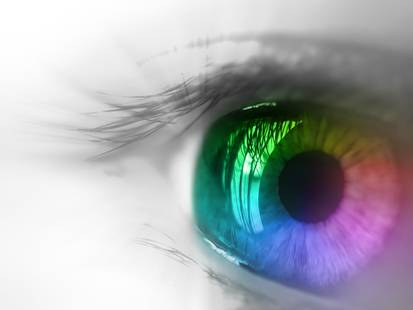
\includegraphics[scale=1]{bilder/oye.jpg}
\end{center}




%%%%%%%%%%%%%%%%%%%%%%%%%%%%%%%%%%%%%%%%%%%%%%%%%%%%%%%%%%%%%%%%%%%%%%%%
\newpage
% Sammendragsside på norsk
%%%%%%%%%%%%%%%%%%%%%%%%%%%%%%%%%%%%%%%%%%%%%%%%%%%%%%%%%%%%%%%%%%%%%%%%

\thispagestyle{fancy}{
\cfoot{\textbf{\small Høgskolen tar ikke ansvar for denne studentrapportens resultater og konklusjoner}\\

\includegraphics[scale=1]{logobilder/pi.jpg} Avdeling for teknologiske fag}}

\label{Sammendrag}\pdfbookmark[1]{Sammendrag}{Sammendrag}

\RapportFra  \\
\begin{tabbing}
    \textbf{Emne: }   \= \textit{\Emnekode { } \Emne }\\
    \textbf{Tittel: } \> \textit{\Tittel}
\end{tabbing}
\noindent\\
Rapporten utgjør en del av vurderingsgrunnlaget i emnet.
\noindent\\
\begin{tabbing}
    \noindent \textbf{Prosjektgruppe: }     \=
    \textit{\Gruppe }\hspace{35mm}          \=
    \textbf{Tilgjengelighet: }\hspace{3mm}  \=
    \textit{Åpen}              \\
    \noindent                  \\
    \textbf{Gruppedeltakere:}  \\
    \textit{André Skare Berg}  \\
    \textit{Espen Løkseth}     \\
    \textit{Matias Wilhelmsen} \\
    \textit{Kristian Torsvik}  \\
    \noindent                  \\
    \textbf{Hovedveileder:}    \> \textit{\Hovedveileder} \> \textbf{Sensor:}          \> \textit{\Sensor} \\
    \textbf{Biveileder: }      \> \textit{\Biveileder}    \> \textbf{Prosjektpartner:} \> \textit{\Prosjektpartner}
\end{tabbing}

\noindent\\
\textbf{Godkjent for arkivering: }\hrulefill \\

\noindent\storboks{
\textbf{Sammendrag:}

Prosjektet i \Emne{} inneholder bygging og oppkopling av et transportbåndsystem med fyllestasjon og enkel sortering. Systemet er styrt av en Siemens S7-300 PLS med tilhørende skjermbasert brukergrensesnitt.
%
Datamatriser brukes for å bestemme fylling og sortering av beholderne på båndet. Det benyttes en vision-sensor av typen DVT Legend 530 til gjenkjenning av matrisene.
%
Oppgaven fokuserer spesielt  på maskinsikkerhet. Som følge av klemfare ved bruk av maskinen, er det benyttet en sikkerhetsmonitor med tilhørende lysgardin. Denne innretningen er montert for å hindre  at uønskede gjenstander kommer inn i farlig område.
%
%Transportbåndet er bygd med tanke på senere bruk og utvidelser.
Materialvalget er av en slik kvalitet at modellen tåler lang tids bruk og ombygging. Modellen er også bygd slik at materiellet enkelt kan byttes ut eller flyttes.
%
Anlegget fungerer  i henhold til systembeskrivelsen.
%
Dataverktøy som gruppen har benyttet i prosjektet er \LaTeXe{} ved hjelp av MiK\TeX{} og \TeX nicCenter, Autodesk AutoCAD, DVT FrameWork, MS Project, Visio, Office-pakken, Siemens Simatic Step 7 og WinCC.\\
}

%%%%%%%%%%%%%%%%%%%%%%%%%%%%%%%%%%%%%%%%%%%%%%%%%%%%%%%%%%%%%%%%%%%%%%%%
\newpage
% Eventuell sammendragsside på engelsk
%%%%%%%%%%%%%%%%%%%%%%%%%%%%%%%%%%%%%%%%%%%%%%%%%%%%%%%%%%%%%%%%%%%%%%%%

\thispagestyle{fancy}{
\lhead{\hspace*{-23mm}
\includegraphics[width=54mm]{logobilder/svart_logo.jpg}\\
\Large \textbf{Telemark University College}\\
\normalfont \normalsize\textbf{Faculty of Technology}\\
Bachelor of Science}
\cfoot{\textbf{\small TUC takes no responsibility for the results and conclusions in this student journal}\\

\includegraphics[scale=1]{logobilder/pi.jpg} Faculty of Technology}}

\label{Summary}\pdfbookmark[1]{Summary}{Summary}

\textbf{\MakeUppercase{Journal from 6$^\text{TH}$ semester project spring 2011}}  \\
\begin{tabbing}
    \textbf{Course: }   \= \textit{\Emnekode { } \Emne }\\
    \textbf{Title: }    \> \textit{\Tittel}
\end{tabbing}
\noindent\\
This journal is a part of the evaluation result for the course.
\noindent\\
\begin{tabbing}
    \noindent \textbf{Project group: \hspace{6mm}} \= \textit{\Gruppe }\hspace{35mm}   \=
    \textbf{Availability: \hspace{9mm}}            \= \textit{Open}            \\
    \noindent                   \\
    \textbf{Group participants:}\\
    \textit{André Skare Berg}   \\
    \textit{Espen Løkseth}      \\
    \textit{Matias Wilhelmsen}  \\
    \textit{Kristian Torsvik}   \\
    \noindent                   \\
    \textbf{Mentor:}            \> \textit{\Hovedveileder} \> \textbf{Sensor:}          \> \textit{\Sensor} \\
    \textbf{Assisting mentor: } \> \textit{\Biveileder}    \> \textbf{Project partner:} \> \textit{\Prosjektpartner}
\end{tabbing}

\noindent\\
\textbf{Approved: }\hrulefill \\

\noindent\storboks{
\textbf{Summary:}

This project, related to the class «\Emne» involves the construction of a conveyor belt model, with a loading station for  bulk. The conveyor belt model is controlled by a Siemens S7-300 PLS with a corresponding screen-based control system.
%
%Anlegget fungerer tilfredsstillende  i henhold til systembeskrivelsen.
%
Data matrices are used to determine the type and amount of bulk to be loaded into the containers. A vision sensor, DVT Legend 530, has been used for code recognition. The code also determines which platform the containers are directed to.
%
%The assignment has had a particular focus on machine safety. As a result of hazardous areas, a light guard has been implemented at the entrance of the tunnel in order to prevent injury.
The assignment has focused on machine safety.  To prevent access to hazardous areas, a safety monitor connected to a light guard has been implemented.
%
%Transportbåndet er bygd med tanke på senere bruk og utvidelser.
%Materialvalget er av en slik kvalitet at modellen tåler lang tids bruk og ombygging. Modellen er også bygd slik at materiellet enkelt kan byttes ut eller flyttes.
%
%The conveyor belt model has been constructed with concern of later use and scalability.
%The material and design for the model has been chosen accordingly.
%
All the materials used in the construction are selected for long-term use and scalability.
%
The project resulted in a system fulfilling the spesifictions defined by the assignment.
%
%
Computer tools used in this project are \LaTeXe{} with MiK\TeX{} and \TeX nicCenter, Autodesk AutoCAD, DVT FrameWork, MS Project, Visio, the Office suite, Siemens Simatic Step 7 and WinCC.\blanklines{1}
}





\setlength{\textheight}{\normalTeksthoyde}
\clearpage\pagenumbering{arabic}
\NormalTopp
\thispagestyle{fancy}{\rhead{\toppfont\currenttitle}}
\pdfbookmark[1]{Forord}{Forord*} % Legg til i PDF-bokmerker
\setcounter{page}{2}
%%%%%%%%%%%%%%%%%%%%%%%%%%%%%%%%%%%%%%%%%%%%%%%%%%%%%%%%%%%%%%%%%%%%%%%%
\section*{Forord}
%%%%%%%%%%%%%%%%%%%%%%%%%%%%%%%%%%%%%%%%%%%%%%%%%%%%%%%%%%%%%%%%%%%%%%%

%%%%%%%%%%%%%%%%%%%%%%%%%%%%%%%%%%%%%%%%%%%%%%%%%%%%%%%%%%%%%%%%%%%%%%%%
\subfile{forord.tex}
%%%%%%%%%%%%%%%%%%%%%%%%%%%%%%%%%%%%%%%%%%%%%%%%%%%%%%%%%%%%%%%%%%%%%%%%








\clearpage
\NormalTopp
\pdfbookmark[1]{Nomenklaturliste}{Nomenklaturliste}
%%%%%%%%%%%%%%%%%%%%%%%%%%%%%%%%%%%%%%%%%%%%%%%%%%%%%%%%%%%%%%%%%%%%%%%%
% Nomenklaturliste
%%%%%%%%%%%%%%%%%%%%%%%%%%%%%%%%%%%%%%%%%%%%%%%%%%%%%%%%%%%%%%%%%%%%%%%%

%%%%%%%%%%%%%%%%%%%%%%%%%%%%%%%%%%%%%%%%%%%%%%%%%%%%%%%%%%%%%%%%%%%%%%%%
\subfile{nomenklaturliste}
%%%%%%%%%%%%%%%%%%%%%%%%%%%%%%%%%%%%%%%%%%%%%%%%%%%%%%%%%%%%%%%%%%%%%%%%








\renewcommand*\contentsname{Innholdsfortegnelse}
\let\a\contentsname
\renewcommand*\contentsname{\MakeUppercase{\a}}
\newpage
%%%%%%%%%%%%%%%%%%%%%%%%%%%%%%%%%%%%%%%%%%%%%%%%%%%%%%%%%%%%%%%%%%%%%%%%
% Innholdsliste
%%%%%%%%%%%%%%%%%%%%%%%%%%%%%%%%%%%%%%%%%%%%%%%%%%%%%%%%%%%%%%%%%%%%%%%%
\thispagestyle{fancy}{
\rhead{\toppfont\a}}
\pdfbookmark[1]{\a}{toc} % Legg til toc i PDF-bokmerker
%%%%%%%%%%%%%%%%%%%%%%%%%%%%%%%%%%%%%%%%%%%%%%%%%%%%%%%%%%%%%%%%%%%%%%%%
\tableofcontents
%%%%%%%%%%%%%%%%%%%%%%%%%%%%%%%%%%%%%%%%%%%%%%%%%%%%%%%%%%%%%%%%%%%%%%%%




\clearpage
\renewcommand{\sectionmark}[1]{
\markboth{\toppfont\thesection \ #1}{}}






%################################################################################
%###################  Hoveddelen av rapporten  ##################################
%################################################################################
%
%          Alle disse subfilene har "<normal"> formatering.
%
%################################################################################

%%%%%%%%%%%%%%%%%%%%%%%%%%%%%%%%%%%%%%%%%%%%%%%%%%%%%%%%%%%%%%%%%%%%%%%%
\subfile{innledning}
%%%%%%%%%%%%%%%%%%%%%%%%%%%%%%%%%%%%%%%%%%%%%%%%%%%%%%%%%%%%%%%%%%%%%%%%


%%%%%%%%%%%%%%%%%%%%%%%%%%%%%%%%%%%%%%%%%%%%%%%%%%%%%%%%%%%%%%%%%%%%%%%%
\subfile{systembeskrivelse}
%%%%%%%%%%%%%%%%%%%%%%%%%%%%%%%%%%%%%%%%%%%%%%%%%%%%%%%%%%%%%%%%%%%%%%%%


%%%%%%%%%%%%%%%%%%%%%%%%%%%%%%%%%%%%%%%%%%%%%%%%%%%%%%%%%%%%%%%%%%%%%%%%
\subfile{maskinvare}
%%%%%%%%%%%%%%%%%%%%%%%%%%%%%%%%%%%%%%%%%%%%%%%%%%%%%%%%%%%%%%%%%%%%%%%%


%%%%%%%%%%%%%%%%%%%%%%%%%%%%%%%%%%%%%%%%%%%%%%%%%%%%%%%%%%%%%%%%%%%%%%%%
\subfile{mekanisk}
%%%%%%%%%%%%%%%%%%%%%%%%%%%%%%%%%%%%%%%%%%%%%%%%%%%%%%%%%%%%%%%%%%%%%%%%


%%%%%%%%%%%%%%%%%%%%%%%%%%%%%%%%%%%%%%%%%%%%%%%%%%%%%%%%%%%%%%%%%%%%%%%%
\subfile{feltbuss}
%%%%%%%%%%%%%%%%%%%%%%%%%%%%%%%%%%%%%%%%%%%%%%%%%%%%%%%%%%%%%%%%%%%%%%%%


%%%%%%%%%%%%%%%%%%%%%%%%%%%%%%%%%%%%%%%%%%%%%%%%%%%%%%%%%%%%%%%%%%%%%%%%
\subfile{vision}
%%%%%%%%%%%%%%%%%%%%%%%%%%%%%%%%%%%%%%%%%%%%%%%%%%%%%%%%%%%%%%%%%%%%%%%%


%%%%%%%%%%%%%%%%%%%%%%%%%%%%%%%%%%%%%%%%%%%%%%%%%%%%%%%%%%%%%%%%%%%%%%%%
\subfile{pls-og-hmi}
%%%%%%%%%%%%%%%%%%%%%%%%%%%%%%%%%%%%%%%%%%%%%%%%%%%%%%%%%%%%%%%%%%%%%%%%


%%%%%%%%%%%%%%%%%%%%%%%%%%%%%%%%%%%%%%%%%%%%%%%%%%%%%%%%%%%%%%%%%%%%%%%%
\subfile{konklusjon}
%%%%%%%%%%%%%%%%%%%%%%%%%%%%%%%%%%%%%%%%%%%%%%%%%%%%%%%%%%%%%%%%%%%%%%%%


%################################################################################
%################################################################################
%################################################################################






%\bibliographystyle{ieeetr}
%\bibliographystyle{unsrt}
\bibliographystyle{logobilder/espen}

%%%%%%%%%%%%%%%%%%%%%%%%%%%%%%%%%%%%%%%%%%%%%%%%%%%%%%%%%%%%%%%%%%%%%%%%%%
 \Referanser
%%%%%%%%%%%%%%%%%%%%%%%%%%%%%%%%%%%%%%%%%%%%%%%%%%%%%%%%%%%%%%%%%%%%%%%%%%

\bibliography{referanser}













%%%%%%%%%%%%%%%%%%%%%%%%%%%%%%%%%%%%%%%%%%%%%%%%%%%%%%%%%%%%%%%%%%%%%%%%%
\Vedlegg
%%%%%%%%%%%%%%%%%%%%%%%%%%%%%%%%%%%%%%%%%%%%%%%%%%%%%%%%%%%%%%%%%%%%%%%%%


\begin{enumerate}[leftmargin=*, label={Vedlegg \Alph*}, align=left]
    \renewcommand{\theenumi}{\Alph{enumi}}
    \let\c\item\renewcommand{\item}[1]{\c\label{#1}}

     \item{ved:framdrift}			   Framdriftsplan. % A
     \item{ved:wbs}					   WBS.            % B
     \item{ved:oppgavetekst}		   Oppgavetekst.   % C
     \item{ved:ob1}                    PLS: Hovedblokk, OB1 (FBD).           % D
     \item{ved:sfc}					   PLS: Blokk som styrer automatisk sekvens, FB1 (SFC).    % E
	\item{ved:hjelp}	               PLS: Blokk som håndterer sikkerhetsmodus, kamerasignaler og manuell kjøring, FC1 (FBD).  % F
	\item{ved:frekvensomformerprogram} PLS: Blokk for styring av frekvensomformer, FB2 (FBD).  % G
	\item{ved:skjema}	               Koplingsskjema med tilhørende koplingstabeller.         % H
	\item{ved:materialliste}	       Materialliste.         % I
\end{enumerate}









\end{document}
